\documentclass[a4paper]{article}
\usepackage[english]{babel}
\usepackage{multicol}
\usepackage{amsmath}
\usepackage{amsfonts}
\usepackage{amssymb}
\usepackage[font=scriptsize]{caption}
\usepackage{parskip}
\usepackage[a4paper, margin=1in, total={6in, 8in}]{geometry}
\usepackage{titling}
\usepackage{subcaption}
\usepackage{float}
\usepackage{placeins}
\usepackage{graphicx}
\usepackage[backend=biber,style=numeric]{biblatex}
\addbibresource{references.bib}

\parskip = 6pt plus 2pt minus 2pt
\setlength{\droptitle}{-2cm}

\title{HW9 - Computer Simulation II}
\author{Schewtschik, Guilherme (3748052)}
\date{\today}

\begin{document}
\maketitle

\section{}
Using the following function to reweigh the observables:

\begin{verbatim}
def reweight_moments(energies, magnetizations, L,
                     beta0, beta_values):
    V = L * L

    m = magnetizations / V

    absm = np.abs(m)

    m2 = m ** 2
    m4 = m ** 4

    results = []

    for beta in beta_values:

        delta = beta - beta0

        # logarithmic weights improve numerical stability
        logw = -delta * energies
        logw -= np.max(logw)

        w = np.exp(logw)

        Z = np.sum(w)

        mean_absm = np.sum(w * absm) / Z
        mean_m2 = np.sum(w * m2) / Z
        mean_m4 = np.sum(w * m4) / Z

        results.append(
            {
                "beta": beta,
                "absm": mean_absm,
                "m2": mean_m2,
                "m4": mean_m4,
            }
        )

    return pd.DataFrame(results)
\end{verbatim}

\newpage
We obtain the following graph:

\begin{figure}[ht]
    \centering
    
\includegraphics[width=0.85\linewidth]{figures/reweighting_magnetisation.png}
    \caption{Magnetizations.}
    \label{fig:mags}
\end{figure}

We can see the reweighted observables stay close to the actual simulation and display the expected behaviour becoming small below $\beta_c$ and approaching $1$ above the critical 
temperature, we also see that the higher powers of the magnetization stay closer to zero in the unorderd phase and need a higher 
temperature to truly magnetize.
The size scaling shows that with bigger lattice sizes this effect is even more exagerated, where the different powers of the 
magnetization stay separate for longer in the $L=32$ case.

\section{}

Simulating the potts model for $L=16,32,64 \& 128$, and using the binning method to estimate the auto correlation time

\begin{figure}[ht]
    \centering
    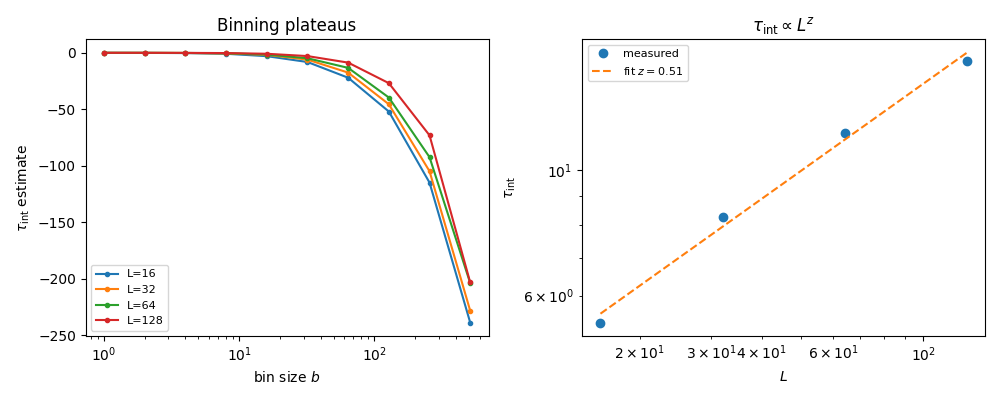
\includegraphics[width=0.85\linewidth]{figures/q2.png}
    \caption{Autocorrelation time.}
    \label{fig:Autotime}
\end{figure}

The binning plateaus confirm that $\tau_{int}$ is small for all system sizes. A log-log fit of $\tau_{int}$ and $L$ 
yields the value for $z \approx 0.51$. The fitted $z$ value is noticeably larger than the value observed for the Wolff 
algorithm on the 2D Ising model of $z \approx 0.25$, which is expected.
\printbibliography


\end{document}